\documentclass[usenames,dvipsnames]{beamer}

\mode<presentation> {%
	\usetheme{Frankfurt}
}

% \usepackage{times}
\usepackage{amsmath,amssymb}
\usepackage[english]{babel}
\usepackage[utf8]{inputenc}
% \usepackage[latin1]{inputenc}

\usepackage{fancybox}
\usefonttheme[onlymath]{serif}
\boldmath

\usepackage{scalefnt}
\usepackage{ragged2e}
\usepackage{graphics}
\usepackage{url}
\usepackage{graphicx}
\usepackage{mathrsfs}
\usepackage{amsfonts}
\usepackage[authoryear,round]{natbib}
\usepackage{multirow}

\usepackage[group-separator={,}]{siunitx}
\usepackage{caption}
\usepackage{pbox}
\usepackage{tabularx}
\usepackage{booktabs}


% \usepackage{color}
% \usepackage[dvipsnames]{xcolor}
% \usepackage[x11names, rgb, dvipsnames]{xcolor}

\graphicspath{{../figures/}{../figures/workshop_data_science/}}

\usepackage{tikz}
\usetikzlibrary{shapes}
\usetikzlibrary{arrows}


\captionsetup[figure]{labelformat=empty}% redefines the caption setup of the figures environment in the beamer class.

\DeclareMathOperator{\ypred}{y_{pred}}
\DeclareMathOperator{\ytrue}{y_{true}}

\DeclareMathOperator{\rank}{rank}
\DeclareMathOperator{\cov}{cov}

\DeclareMathOperator{\TP}{TP}
\DeclareMathOperator{\TN}{TN}
\DeclareMathOperator{\FP}{FP}
\DeclareMathOperator{\FN}{FN}
\DeclareMathOperator{\FPR}{FPR}
\DeclareMathOperator{\AUC}{AUC}
\DeclareMathOperator{\TNR}{TNR}
\DeclareMathOperator{\TNA}{TNA}
\DeclareMathOperator{\TPA}{TPA}
\DeclareMathOperator{\TPR}{TPR}

\DeclareMathOperator{\Precision}{Precision}
\DeclareMathOperator{\Recall}{Recall}
\DeclareMathOperator{\InvPrecision}{Inverse\ Precision}
\DeclareMathOperator{\InvRecall}{Inverse\ Recall}
\DeclareMathOperator{\Accuracy}{Accuracy}

\DeclareMathOperator{\calls}{calls}
\DeclareMathOperator{\etime}{time}
\DeclareMathOperator{\sms}{sms}
\DeclareMathOperator{\contacts}{contacts}

\DeclareMathOperator{\ein}{in}
\DeclareMathOperator{\out}{out}

\DeclareMathOperator{\low}{low}
\DeclareMathOperator{\high}{high}

\DeclareMathOperator{\train}{train}
\DeclareMathOperator{\test}{test}

\DeclareMathOperator{\Betainc}{\Beta_{\operatorname{inc}}}

\DeclareMathOperator{\incalls}{incalls}
\DeclareMathOperator{\outcalls}{outcalls}
\DeclareMathOperator{\insms}{insms}
\DeclareMathOperator{\outsms}{insms}
\DeclareMathOperator{\intime}{outtime}
\DeclareMathOperator{\outtime}{outtime}
\DeclareMathOperator{\incontacts}{incontacts}
\DeclareMathOperator{\outcontacts}{outcontacts}

\DeclareMathOperator{\incallslow}{incallslow}
\DeclareMathOperator{\outcallslow}{outcallslow}
\DeclareMathOperator{\insmslow}{insmslow}
\DeclareMathOperator{\outsmslow}{insmslow}
\DeclareMathOperator{\intimelow}{outtimelow}
\DeclareMathOperator{\outtimelow}{outtimelow}
\DeclareMathOperator{\incontactslow}{incontactslow}
\DeclareMathOperator{\outcontactslow}{outcontactslow}

\DeclareMathOperator{\incallshigh}{incallshigh}
\DeclareMathOperator{\outcallshigh}{outcallshigh}
\DeclareMathOperator{\insmshigh}{insmshigh}
\DeclareMathOperator{\outsmshigh}{insmshigh}
\DeclareMathOperator{\intimehigh}{outtimehigh}
\DeclareMathOperator{\outtimehigh}{outtimehigh}
\DeclareMathOperator{\incontactshigh}{incontactshigh}
\DeclareMathOperator{\outcontactshigh}{outcontactshigh}

\DeclareMathOperator{\neigh}{Neigh}

\DeclareMathOperator{\dir}{dir}
\DeclareMathOperator{\cat}{cat}

\DeclareMathOperator{\ego}{ego}

\DeclareMathOperator{\logit}{logit}

\DeclareMathOperator{\Betadist}{Beta}
\DeclareMathOperator{\Binomial}{Bin}


% \DeclareMathOperator{\ego}{Ring}
% \DeclareMathOperator{\cat}{Cat}

\newcommand{\Beta}{B}

\newcommand{\mathA}{\mathcal{A}}
\newcommand{\mathB}{\mathcal{B}}
\newcommand{\mathC}{\mathcal{C}}
\newcommand{\mathG}{\mathcal{G}}
\newcommand{\mathP}{\mathcal{P}}

\newcommand{\TP}{\operatorname{TP}}
\newcommand{\TN}{\operatorname{TN}}
\newcommand{\FP}{\operatorname{FP}}
\newcommand{\TPR}{\operatorname{TPR}}
\newcommand{\FPR}{\operatorname{FPR}}
\newcommand{\AUC}{\operatorname{AUC}}

\newcommand{\closeopen}[2]{\left[ #1, #2 \right)}

\usepackage{array}
\newcolumntype{L}[1]{>{\raggedright\let\newline\\\arraybackslash\hspace{0pt}}m{#1}}
\newcolumntype{C}[1]{>{\centering\let\newline\\\arraybackslash\hspace{0pt}}m{#1}}
\newcolumntype{R}[1]{>{\raggedleft\let\newline\\\arraybackslash\hspace{0pt}}m{#1}}

\beamertemplatenavigationsymbolsempty

%%%%%%%%%%%%%%%%%%%%%%%%%%%%%%%%%%%%%%%%%%%%%%%%%%%%%%%%%%%%%%%%%%%%%%%%%%%%%%%%%%%%%%%%%%%%%%%%%%%%%%%%%%%%
%%%%%%%%%%%%%%%%%%%%%%%%%%%%%%%%%%%%%%%%%%%%%%%%%%%%%%%%%%%%%%%%%%%%%%%%%%%%%%%%%%%%%%%%%%%%%%%%%%%%%%%%%%%%

\title[Predictors for Income Inference]
{Featurization Methods and Predictors for Income Inference based on Communication Patterns}

\author{%
	{Carlos~Sarraute}\inst{}
}

\institute{%
	\inst{}Grandata Labs, Buenos Aires \& San Francisco \\
	\texttt{charles@grandata.com}
}

\bigskip

\date[MOTIf]{MOTIf Meeting \\ June 7-8, 2018}


%\setbeamertemplate{footline}[text line]{\bf \insertshortauthor \hfill \insertshorttitle \hfill \insertframenumber/29}
\setbeamertemplate{footline}[text line]{\hfill \insertframenumber / 27}

\AtBeginSection[]
{%
  \begin{frame}<beamer>{Agenda}
    \tableofcontents[currentsection]
  \end{frame}
}
  
%%%%%%%%%%%%%%%%%%%%%%%%%%%%%%%%%%%%%%%%%%%%%%%%%%%%%%%%%%%%%%%%%%%%%%%%%%%%%%%%%%%%%%%%%%%%%%%%%%%%%%%%%%%%
%%%%%%%%%%%%%%%%%%%%%%%%%%%%%%%%%%%%%%%%%%%%%%%%%%%%%%%%%%%%%%%%%%%%%%%%%%%%%%%%%%%%%%%%%%%%%%%%%%%%%%%%%%%%
%%%%%%%%%%%%%%%%%%%%%%%%%%%%%%%%%%%%%%%%%%%%%%%%%%%%%%%%%%%%%%%%%%%%%%%%%%%%%%%%%%%%%%%%%%%%%%%%%%%%%%%%%%%%
\begin{document}


\begin{frame}
\titlepage
\end{frame}



%%%%%%%%%%%%%%%%%%%%%%%%%%%%%%%%%%%%%%%%%%%%%%%%%%%%%%%%%%%%%%%%%%%%%%%%%%%%%%%%%%%%%%%%%%%%%%%%%%%%%%%%%%%%
\section{Introduction}
%%%%%%%%%%%%%%%%%%%%%%%%%%%%%%%%%%%%%%%%%%%%%%%%%%%%%%%%%%%%%%%%%%%%%%%%%%%%%%%%%%%%%%%%%%%%%%%%%%%%%%%%%%%%

\begin{frame}{Presentation}

\begin{block}{About Grandata Labs}
\begin{itemize}

\item Founded in 2012

\item Research and Data Science team:
\begin{itemize}
\item 10 persons, based in Buenos Aires \& San Francisco
\item Graduates \& PhDs from University of Buenos Aires \\ $\in$ Computer Sc., Physics, Mathematics
\end{itemize}

\item Investigating Human Dynamics
\begin{itemize}
\item Using ``Big Data'' to analyze social networks and human behavior.
\item Integrating banking and cellphone data.
\item Characterize users and predict user actions.
\end{itemize}

\end{itemize}

\end{block}
\end{frame}



\begin{frame}{Our Scientific Collaborations}
\begin{block}{Scientific Partners}
\begin{itemize}
\item Aline, Artur, Humberto, Jussara, Marton (MOTIf)
\medskip
\item Maria Oskarsdottir, Bart Baesens (KU Leuven)
\begin{itemize}
\item Influence of graph construction
\end{itemize}
\medskip
\item Hernan Makse (City College of New York) 
\begin{itemize}
\item Characterization of humans in the graph
\end{itemize}
\medskip
\item Sandy Pentland and Human Dynamics team (MIT)
\item Marta Gonzalez and Human Mobility team (MIT)
\item Fundación Mundo Sano, Fundacion Bunge \& Born
\end{itemize}
\end{block}


{\tiny 
\nocite{leo2015socioeconomic}
\nocite{sarraute2015city}
\nocite{sarraute2014}
}
\end{frame}


\begin{frame}{Summary}

\begin{itemize}

\begin{block}{Objective}
Compare methods for the \textbf{inference of socioeconomic status} in the communication graph.
\end{block}
\medskip

\pause

\item Use 2 data sources:
\begin{itemize}
\item Call Detail Records (CDRs) from the operator allow us to construct a social graph.
\item Banking reported income for a subset of clients obtained from a large bank.
\end{itemize} 

\item We construct an \textcolor{blue}{inference algorithm} that allows us to predict the socioeconomic status of users.

\item We compare it with standard machine learning techniques using growing set of features from nodes and their network.

\end{itemize}

\end{frame}

\begin{frame}{Datasets}

\begin{block}{Mobile Phone Data Source}

Each CDR \( p \in \mathP \) contains:
\begin{itemize}
\item phone numbers of origin and destination \( \left< p_o, p_d \right> \) \\
 anonymized using a cryptographic hash function
\item starting time \( p_t \), call duration \( p_s \)
\item latitude and longitude of antenna used \( \left< p_y, p_x \right> \) for subset of data.
\end{itemize} 

\end{block}

\pause

\begin{block}{Banking Information}

\begin{itemize}
\item Account balances for over 10 million clients of a bank for a period of 6 months, denoted \( \mathB \). 
\item For each client \( b \in \mathB \) we have his phone number \( b_p \), anonymized with the same hash function used in \( \mathP \).
\item The average income of 6 months \( b_s \).

\end{itemize}


\end{block}

\end{frame}


\begin{frame}{Bank and Telco Matching}

\begin{itemize}

\item Phone numbers in each call $ p_o $ and $ p_d $ are anonymized with the same hash function as the phone number in the bank data, $ b_p $.

\item We can match users to their unique phone to create the social graph:
$$ G = \mathP \bowtie_{_{p_o = b_p}} \mathB \bowtie_{_{p_d = b_p}} \mathB $$

\item \( \forall g \in G \) we have its phone number \( g_p \),  its average income over 6 months \( g_s \), and its age \( g_a \).

\item This graph has a total of \num{2027554} nodes with \num{5044976} edges, which represent \num{29599762} calls and \num{5476783} text messages.
\end{itemize}

\end{frame}



%%%%%%%%%%%%%%%%%%%%%%%%%%%%%%%%%%%%%%%%%%%%%%%%%%%%%%%%%%%%%%%%%%%%%%%%%%%%%%%%%%%%%%%%%%%%%%%%%%%%%%%%%%%%
\section{Income Prediction}
%%%%%%%%%%%%%%%%%%%%%%%%%%%%%%%%%%%%%%%%%%%%%%%%%%%%%%%%%%%%%%%%%%%%%%%%%%%%%%%%%%%%%%%%%%%%%%%%%%%%%%%%%%%%

\begin{frame}{What do we use?}

\centering

\begin{LARGE}
Individual features~?

\bigskip

or

\bigskip
\medskip

Network topology~??
\end{LARGE}
\end{frame}


\begin{frame}{Income Homophily}

\begin{figure}[h]
\begin{center}
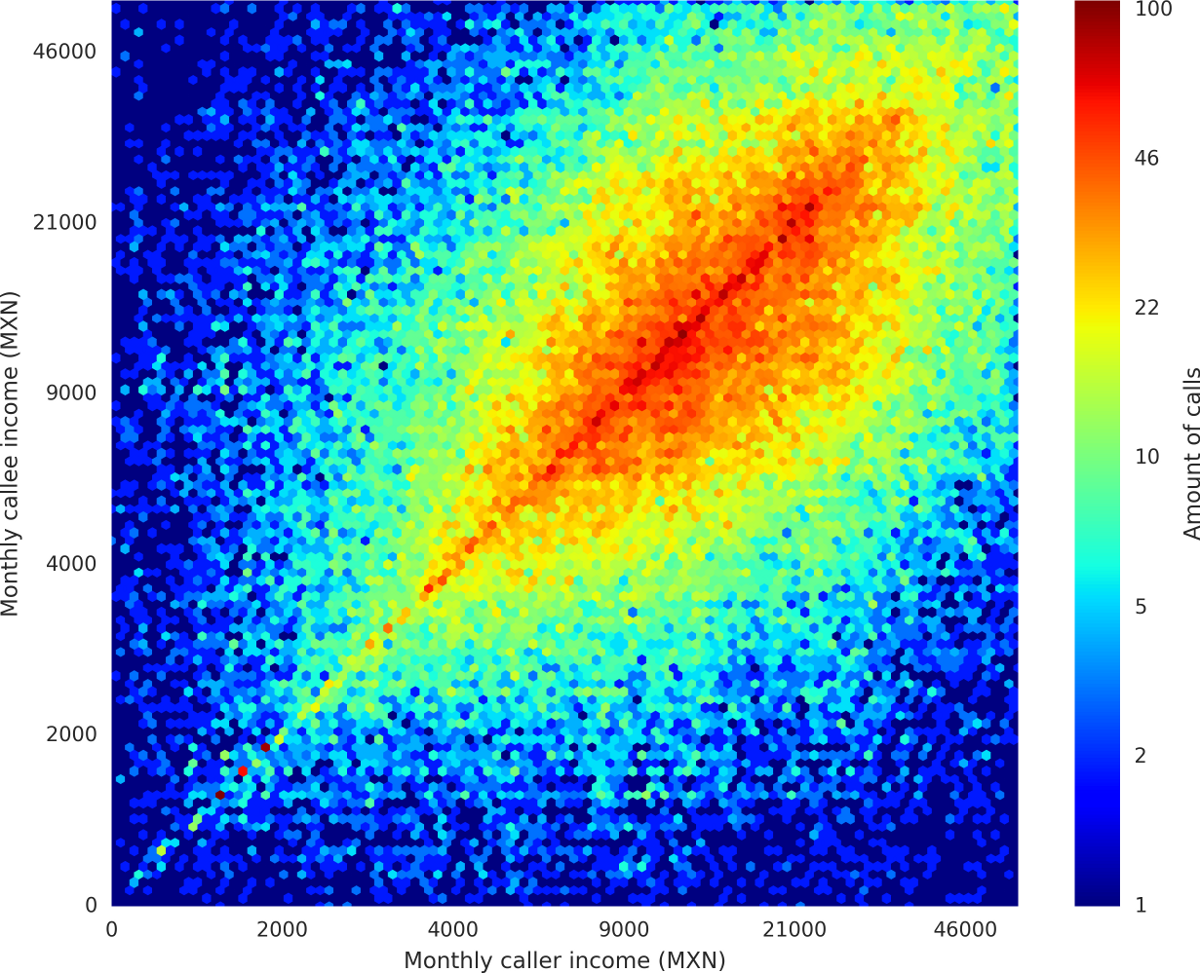
\includegraphics[width=0.7\columnwidth]{Homophily_income_origin_target_low.png}
\caption{Number of calls between users, according to their monthly income \\
\medskip
{\small Similar to homophily with respect to age in~\cite{brea2014}.}
}
\label{homophily_heatmap}
\end{center}
\end{figure}
\end{frame}

\begin{frame}{What do we predict?}

Instead of predicting the exact value of a user's income, our strategy is to distinguish between 2 categories:
\begin{itemize}
\item $R_1 = \closeopen{1000}{6300}$ i.e.\ low income
\item $R_2 = \closeopen{6300}{\infty}$ i.e.\ high income
\end{itemize} 

\bigskip

We place users into two distinct groups $ H_1, H_2 \subseteq G$:
\[
	g \in H_i \iff g_s \in R_i
\]

\end{frame}


%%%%%%%%%%%%%%%%%%%%%%%%%%%%%%%%%%%%%%%%%%%%%%%%%%%%%%%%%%%%%%%%%%%%%%%%%%%%%%%%%%%%%%%%%%%%%%%%%%%%%%%%%%%%
\section{Bayesian Predictor}
%%%%%%%%%%%%%%%%%%%%%%%%%%%%%%%%%%%%%%%%%%%%%%%%%%%%%%%%%%%%%%%%%%%%%%%%%%%%%%%%%%%%%%%%%%%%%%%%%%%%%%%%%%%%


\begin{frame}{Bayesian inference}

\begin{itemize}
\item Reason with \textbf{uncertainty}.
\bigskip
\item Philosophy: treat anything uncertain as random, described by a probability distribution.
\bigskip
\item Given observations, we want to infer the best parameters of the probability distribution.

\end{itemize}
\end{frame}






\begin{frame}{Motivation}

\begin{columns}
\begin{column}{0.49\textwidth}

\begin{figure}[h]
\begin{center}
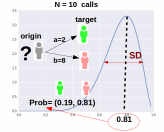
\includegraphics[width=\columnwidth]{distribucion1.png}
\end{center}
\end{figure}
\end{column}

\begin{column}{0.49\textwidth}

\begin{figure}[h]
\begin{center}
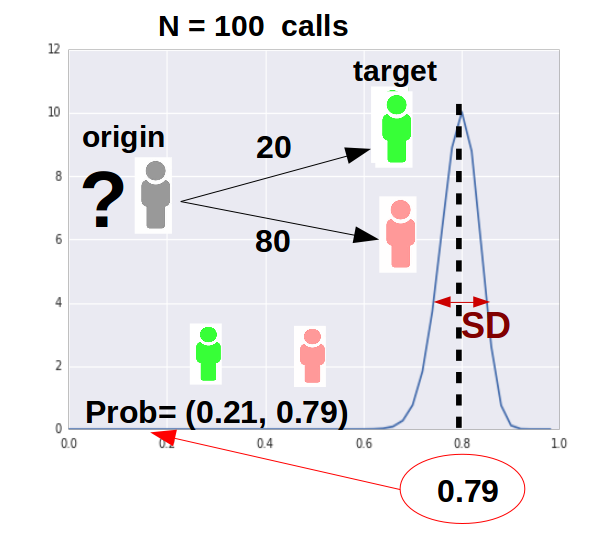
\includegraphics[width=\columnwidth]{distribucion2.png}
\end{center}
\end{figure}

\end{column}
\end{columns}

\medskip

The frequency of calls (to category 1 and 2) loses information.

We want to compare distributions.

\end{frame}



\begin{frame}{Beta Distribution}

We define \(\Beta^j\) as the Beta probability distribution function for each user:
\begin{equation}
	\Beta^j \left( x; \alpha^j, \beta^j \right) = \frac{1}{\Beta \left( \alpha^j, \beta^j \right)} x^{\alpha^j - 1} \cdot {\left( 1 - x \right)}^{\beta^j - 1}
\label{Beta}
\end{equation}
where $\alpha^j = a^j_1 +1$ and $\beta^j = a^j_2 +1$ are the parameters of the Beta distribution,
and $\Beta$ is the beta function, defined as:
\begin{equation}
\Beta \left( \alpha, \beta \right) =
\frac{\Gamma \! \left( \alpha \right) \cdot \Gamma \! \left( \beta \right)}
{\Gamma \! \left( \alpha + \beta \right)}
\label{Beta}
\end{equation}

We obtain a Beta distribution for the probability of belonging to high income category (for each user).

\end{frame}



\begin{frame}{Determining the category}

	\begin{columns}
		\begin{column}{0.49\textwidth}

\begin{figure}[h]
\begin{center}
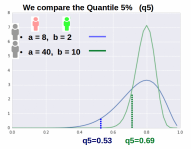
\includegraphics[width=\columnwidth]{distribucion3.png}
% \caption{Tres.}
\end{center}
\end{figure}
\end{column}

\begin{column}{0.49\textwidth}

\begin{figure}[h]
\begin{center}
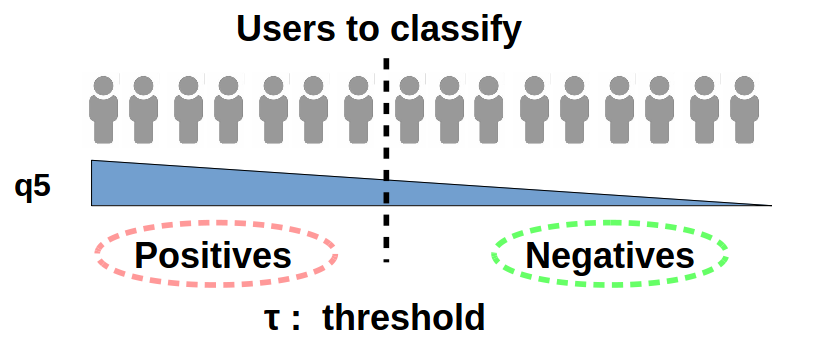
\includegraphics[width=\columnwidth]{distribucion4.png}
% \caption{Cuatro.}
\end{center}
\end{figure}

\end{column}
\end{columns}


\begin{itemize}

\item Find the lowest 5 percentile $q5$ for this probability. 

\item If $q5$ is above threshold $\tau$, we assign user to $H_2$.

\item Take into account both the mean and the broadness (uncertainty) of the distribution. 

\item Category assigned to a user depends on its Beta distribution and on our choice of $\tau$.
\end{itemize}

\end{frame}


\begin{frame}{Evaluation of Performance}

We examine:
\begin{itemize}
\item true positive rate \( \TPR = \TP / \operatorname{P} \)
\item false positive rate \( \FPR = \FP / \operatorname{N} \)
\end{itemize}
Where:
\begin{itemize}
\item $\TP$ (True Positive) is the number of correctly predicted users with high income,
\item $\operatorname{P}$ (Positive) is the total number of users with high income, 
\item $\FP$ (False Positive) is the number of users incorrectly classified as having high income,
\item $\operatorname{N}$ (Negative) is the total number of users with low income.

\end{itemize} 


\end{frame}

\begin{frame}{ROC Curve}

\begin{figure}
\begin{center}
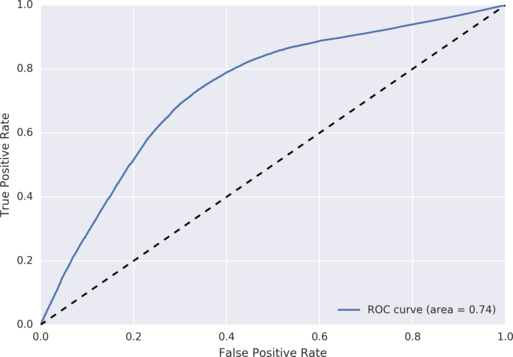
\includegraphics[width=0.7\columnwidth]{ROC_Beta_based_approach_201504.png}
\caption{ROC curve for prediction procedure}
\label{ROC_multiclass}
\end{center}
\end{figure}

We observed an $\AUC = 0.74$ indicating that our predictor is better than a random predictor ($\AUC \simeq 0.50$).

\end{frame}


\begin{frame}{Accuracy}

\begin{figure}[p]
\begin{center}
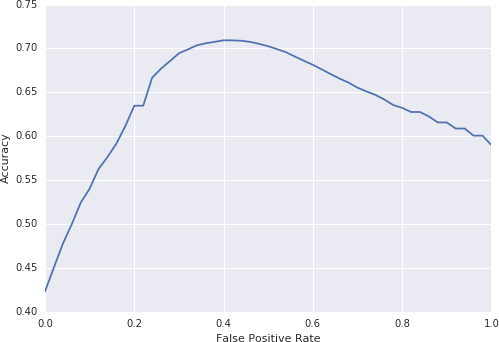
\includegraphics[width=0.7\columnwidth]{accuracy_vs_fpr.png}
\caption{Accuracy as a function of FPR}
\label{fig:accuracy_vs_fpr}
\end{center}
\end{figure}

The best accuracy obtained is \num{0.71} for $\tau = 0.4$.

\end{frame}



%%%%%%%%%%%%%%%%%%%%%%%%%%%%%%%%%%%%%%%%%%%%%%%%%%%%%%%%%%%%%%%%%%%%%%%%%%%%%%%%%%%%%%%%%%%%%%%%%%%%%%%%%%%%
\section{Featurization Methods}
%%%%%%%%%%%%%%%%%%%%%%%%%%%%%%%%%%%%%%%%%%%%%%%%%%%%%%%%%%%%%%%%%%%%%%%%%%%%%%%%%%%%%%%%%%%%%%%%%%%%%%%%%%%%


\begin{frame}{Generation of Graph Features}

For each link $e \in E$ in the graph we have:

\begin{itemize}
	\item \textbf{Origin} of the calls and SMS
	\item \textbf{Destination} of the calls and SMS
	\item \textbf{Calls}: total number of calls
	\item \textbf{Time}: total time (in seconds) of all the calls
	\item \textbf{SMS}: total amount of messages
\end{itemize}

\end{frame}


\begin{frame}{Higher order user data -- $\ego_{n > 1}$ }

\begin{figure}
\centering
\framebox[\columnwidth]{%
	
\begin{tikzpicture}[>=latex,line join=bevel,]
%%
\node (b4) at (58.264bp,80.697bp) [draw,ellipse] {};
  \node (b5) at (107.65bp,46.247bp) [draw,ellipse] {};
  \node (b6) at (134.09bp,46.247bp) [draw,ellipse] {};
  \node (b7) at (183.48bp,80.697bp) [draw,ellipse] {};
  \node (b0) at (183.48bp,124.78bp) [draw,ellipse] {};
  \node (b1) at (158.52bp,150.63bp) [draw,ellipse] {};
  \node (b2) at (107.65bp,159.23bp) [draw,ellipse] {};
  \node (b3) at (64.526bp,134.74bp) [draw,ellipse] {};
  \node (c11) at (64.398bp,30.901bp) [draw,ellipse] {};
  \node (c10) at (36.354bp,54.739bp) [draw,ellipse] {};
  \node (a1) at (92.698bp,86.739bp) [draw,ellipse] {};
  \node (a0) at (133.84bp,129.35bp) [draw,ellipse] {};
  \node (c9) at (21.176bp,85.884bp) [draw,ellipse] {};
  \node (a2) at (139.69bp,78.794bp) [draw,ellipse] {};
  \node (c3) at (140.7bp,18.0bp) [draw,ellipse] {};
  \node (c2) at (220.56bp,85.884bp) [draw,ellipse] {};
  \node (c1) at (205.39bp,54.739bp) [draw,ellipse] {};
  \node (c0) at (220.56bp,119.6bp) [draw,ellipse] {};
  \node (c7) at (205.39bp,150.74bp) [draw,ellipse] {};
  \node (c6) at (64.398bp,174.58bp) [draw,ellipse] {};
  \node (c5) at (101.04bp,187.48bp) [draw,ellipse] {};
  \node (c4) at (140.7bp,187.48bp) [draw,ellipse] {};
  \node (a3) at (152.17bp,91.719bp) [draw,ellipse] {};
  \node (c8) at (21.176bp,119.6bp) [draw,ellipse] {};
  \node (v) at (120.87bp,102.74bp) [draw,fill=gray,ellipse] {v};
  \draw [red,] (v) ..controls (135.03bp,84.728bp) and (135.11bp,84.621bp)  .. (a2);
  \draw [ForestGreen,] (b6) ..controls (138.26bp,28.429bp) and (138.28bp,28.341bp)  .. (c3);
  \draw [blue,] (a1) ..controls (80.328bp,107.82bp) and (76.815bp,113.8bp)  .. (b3);
  \draw [ForestGreen,] (b7) ..controls (166.4bp,55.662bp) and (157.67bp,42.867bp)  .. (c3);
  \draw [blue,] (a0) ..controls (121.21bp,143.76bp) and (120.45bp,144.63bp)  .. (b2);
  \draw [ForestGreen,] (b2) ..controls (87.533bp,166.37bp) and (84.387bp,167.49bp)  .. (c6);
  \draw [ForestGreen,] (b4) ..controls (41.841bp,97.922bp) and (37.585bp,102.39bp)  .. (c8);
  \draw [red,] (v) ..controls (142.36bp,95.175bp) and (142.44bp,95.145bp)  .. (a3);
  \draw [ForestGreen,] (b7) ..controls (199.9bp,97.922bp) and (204.16bp,102.39bp)  .. (c0);
  \draw [blue,] (a0) ..controls (147.71bp,141.31bp) and (147.8bp,141.39bp)  .. (b1);
  \draw [ForestGreen,] (b0) ..controls (195.28bp,138.77bp) and (195.36bp,138.87bp)  .. (c7);
  \draw [ForestGreen,] (b4) ..controls (61.028bp,58.262bp) and (61.616bp,53.483bp)  .. (c11);
  \draw [ForestGreen,] (b2) ..controls (103.48bp,177.05bp) and (103.46bp,177.14bp)  .. (c5);
  \draw [blue,] (a1) ..controls (74.544bp,83.554bp) and (74.414bp,83.531bp)  .. (b4);
  \draw [red,] (v) ..controls (130.88bp,123.29bp) and (130.94bp,123.4bp)  .. (a0);
  \draw [ForestGreen,] (b7) ..controls (195.28bp,66.71bp) and (195.36bp,66.613bp)  .. (c1);
  \draw [blue,] (a0) ..controls (156.36bp,127.28bp) and (160.96bp,126.85bp)  .. (b0);
  \draw [ForestGreen,] (b4) ..controls (46.458bp,66.71bp) and (46.377bp,66.613bp)  .. (c10);
  \draw [blue,] (a3) ..controls (169.4bp,85.652bp) and (169.52bp,85.612bp)  .. (b7);
  \draw [ForestGreen,] (b5) ..controls (87.533bp,39.109bp) and (84.387bp,37.993bp)  .. (c11);
  \draw [ForestGreen,] (b2) ..controls (123.17bp,172.5bp) and (124.91bp,173.98bp)  .. (c4);
  \draw [blue,] (a1) ..controls (99.753bp,67.634bp) and (100.57bp,65.415bp)  .. (b5);
  \draw [blue,] (a2) ..controls (136.61bp,60.878bp) and (136.59bp,60.759bp)  .. (b6);
  \draw [red,] (v) ..controls (100.85bp,91.371bp) and (100.71bp,91.289bp)  .. (a1);
  \draw [blue,] (a1) ..controls (110.72bp,69.108bp) and (116.32bp,63.636bp)  .. (b6);
  \draw [blue,] (a1) ..controls (98.712bp,115.9bp) and (101.69bp,130.32bp)  .. (b2);
  \draw [ForestGreen,] (b7) ..controls (201.88bp,83.271bp) and (202.17bp,83.312bp)  .. (c2);
  \draw [ForestGreen,] (b4) ..controls (39.861bp,83.271bp) and (39.566bp,83.312bp)  .. (c9);
  \draw [ForestGreen,] (b0) ..controls (201.88bp,122.21bp) and (202.17bp,122.17bp)  .. (c0);
%
\end{tikzpicture}


}
\caption{Edges present in the calculation of the \emph{Higher Order User Data} for a certain node $v$. \\
\textcolor{red}{Red} edges represent \emph{User data of order 1},\\
 \textcolor{blue}{Blue} edges represent \emph{User data of order 2}, \\
 \textcolor{ForestGreen}{Green} edges represent \emph{User data of order 3}.}
\label{fig:higherorderuserdata}
\end{figure}


\end{frame}


\begin{frame}{Categorical User Data -- Level $\cat_n$}

We add the information of the income category of the other party in the link to 
edges in $\ego_{n}$ obtaining $\cat_n$:

\begin{columns}
\begin{column}{0.6\textwidth}
\begin{equation*}
\begin{Bmatrix} in \\ out \end{Bmatrix}
\times
\begin{Bmatrix} calls \\ time \\ sms \\ contacts \end{Bmatrix}
\times
\begin{Bmatrix} low \\ high \\ unknown \end{Bmatrix}
\label{eq:matcatuserdata}
\end{equation*}
\end{column}
\begin{column}{0.4\textwidth}
\begin{table}[t]
% \centering
\begin{tabular}{>{\bfseries}l r}
\toprule
Level & Features \\
\midrule
$\ego_1$ & \num{8}  \\
$\ego_2$ & \num{16} \\
$\ego_3$ & \num{24} \\
$\cat_1$ & \num{24} \\
$\cat_2$ & \num{48} \\
$\cat_3$ & \num{72} \\
\bottomrule
\end{tabular}
\end{table}
\end{column}
\end{columns}

\end{frame}



\begin{frame}{Machine Learning methods}

We used \textbf{Logistic Regression} and \textbf{Random Forests}. \\
We performed a grid search to tune hyper-parameters and used 5-fold cross validation.  
\medskip

We measure:
\begin{itemize}
\item \textcolor{Plum}{AUC} = Area under the ROC curve.
\item \textcolor{Plum}{Accuracy} = $(\TP + \TN) / (\operatorname{P} + \operatorname{N})$
\item \textcolor{Plum}{Precision} = $\TP / (\TP + \FP)$
\item \textcolor{Plum}{Recall} = $\TP / \operatorname{P}$
\item \textcolor{Plum}{F1-score} = 
	$ 2 \cdot \frac{1}{ \frac{1}{\mbox{precision}} + \frac{1}{\mbox{recall}} } $
\item \textcolor{Plum}{F4-score} = attaches 4 times more importance to recall as precision
\end{itemize}

\end{frame}



\begin{frame}{Results -- Inner graph}
\begin{table}
{\small 
\begin{tabular*}{\textwidth}{>{\bfseries}l >{\bfseries}l @{\extracolsep{\fill}}>{\hspace{2em}}r r r }
\toprule
Model & Level & AUC & F\textsubscript{1}-score & F\textsubscript{4}-score  \\
\midrule

\multicolumn{2}{>{\bfseries}l}{Random Selection}
& 0.499 & 0.500 & 0.500  \\

\multicolumn{2}{>{\bfseries}l}{Majority Voting}
& 0.681 & 0.721 & 0.712  \\

\multicolumn{2}{>{\bfseries}l}{\textcolor{blue}{Bayesian Algorithm}}
& \textcolor{blue}{\textbf{0.746}} & \textcolor{blue}{\textbf{0.723}} & \textcolor{blue}{\textbf{0.783}}  \\
\midrule

\multirow{5}{*}{LR} &
\textcolor{gray}{$\ego_1$} & \textcolor{gray}{0.536} & \textcolor{gray}{0.574} & \textcolor{gray}{0.619}  \\
& \textcolor{gray}{$\ego_2$} & \textcolor{gray}{0.535} & \textcolor{gray}{0.611} & \textcolor{gray}{0.714} \\
& \textcolor{gray}{$\ego_3$} & \textcolor{gray}{0.569} & \textcolor{gray}{0.550} & \textcolor{gray}{0.528} \\
& $\cat_1$ & 0.686 & 0.714 & \textbf{0.776} \\
& $\cat_2$ & \textbf{0.693} & \textbf{0.718} & 0.772 \\
& $\cat_3$ & 0.692 & 0.714 & 0.758 \\

\midrule

\multirow{5}{*}{RF} &
\textcolor{gray}{$\ego_1$} & \textcolor{gray}{0.548} & \textcolor{gray}{0.549} & \textcolor{gray}{0.550} \\
& \textcolor{gray}{$\ego_2$} & \textcolor{gray}{0.582} & \textcolor{gray}{0.580} & \textcolor{gray}{0.577} \\
& \textcolor{gray}{$\ego_3$} & \textcolor{gray}{0.576} & \textcolor{gray}{0.579} & \textcolor{gray}{0.580} \\
& $\cat_1$ & 0.671 & 0.677 & 0.688 \\
& $\cat_2$ & \textbf{0.714} & \textbf{0.714} & \textbf{0.716} \\
& $\cat_3$ & 0.709 & 0.711 & 0.711 \\
\bottomrule
\end{tabular*}
\caption{Results on \emph{Inner Graph}, which contains only nodes which have at least one neighbour with socioeconomic information. \textbf{LR} corresponds to \emph{Logistic Regression} models, and \textbf{RF} to \emph{Random Forest} models.}
\label{tab:innergraphresults}
}
\end{table}


\end{frame}



\begin{frame}{References}
\justifying%
\scalefont{0.75}
\bibliographystyle{unsrtnat}
\bibliography{../Tesis/bibliography/sna}{}

\end{frame}

\begin{frame}{That's all folks!}
\centering
\begin{huge}
Thank you!
\end{huge}

\bigskip
\bigskip
\begin{Large}


\emph{charles@grandata.com}

\medskip
\emph{@ch4rleston}
\end{Large}

\end{frame}

\end{document}

